% Manuscript for the Journal of Educational Data Mining (JEDM), built with the journal's LaTeX template (class jedm,
% reference style acmtrans). The template files are not part of this directory; BUILD.md says where to obtain them.
% The sections are kept in separate files while the manuscript is written. The supplementary material is an appendix
% after the references, as the journal's instructions ask.
\documentclass[notitlepage,12pt]{jedm}
\usepackage[T1]{fontenc}
\usepackage{url}
\usepackage{graphicx}
\usepackage{booktabs}
\usepackage{array}
\usepackage{tabularx}
\usepackage{seqsplit}
\usepackage{amsmath}
\usepackage{pgfplots}
\pgfplotsset{compat=1.18}
\usepackage{hyperref}
\hypersetup{colorlinks=true, urlcolor=blue, linkcolor=blue, citecolor=blue}

% Figures: the colours are the first two slots of a categorical palette checked for separation under colour-vision
% deficiencies; each series also has a mark of its own, so that the figure can be read in grey.
\definecolor{figc1}{HTML}{2A78D6}
\definecolor{figc2}{HTML}{EB6834}
\definecolor{figband}{HTML}{E8E8E8}

\begin{document}

\title{A keystroke state estimator's 30-second signal changes before code-writing stalls: within 0.025 AUC of
matched pauses in a preregistered holdout}
\date{}
\author{{\large Mikoto Miura}\\Independent Researcher\\ORCID 0009-0000-4196-0508}

\maketitle

\begin{abstract}
Keystroke signals are attractive triggers for timely help if they change before a learner stops producing text. We
tested whether the 30-second change, at the start of a pause, in two signals of a keystroke state estimator with
hand-set coefficients (the probability of its Stuck state and a smoothed friction axis) distinguishes pauses that became
stalls in character production from matched pauses of 2--30~s that did not. The test was preregistered on a random
holdout of an introductory programming dataset, with an equivalence band of $[0.45, 0.55]$ for the AUC set in advance;
a leak had shown that on seen writers the AUC lay inside it, so this is a confirmation, not a test of a prediction that
could fail. In the holdout (139 students), the AUC fell within the band for both signals (0.489 and 0.487; the
false-equivalence rate is at most 5.2\% [Wilson 95\% interval 3.6--7.5\%] among the configurations examined in the
calibration on seen writers, and is not an upper bound over the whole null). The Stuck-state probability is mostly at
the floor of the estimate, and claims about run-up change rely on the friction axis and on the pairs not at the floor.
In explorations outside the registration, changes of the
observed size barely moved the signals on seen writers, and on the holdout, learners on simple keystroke quantities
ranked stalls higher, mainly through less preceding typing. Under a conversion made after the band was set, a
difference at its edge would change the share of trigger firings that fall on stalls by about one point, so on this
input the signals gave no basis for a trigger. Preregistration: \url{https://osf.io/mrkxt}; results:
\url{https://osf.io/uj6cy}; code: [archive to be added before submission].\\

{\parindent0pt
\textbf{Keywords:} keystroke logging, stalls, equivalence testing, preregistration, matched controls, introductory
programming
}
\end{abstract}


\section{Introduction}
\label{sec:intro}

A recurring aim of educational data mining is to recognise, while a learner is working, the moment at which help would
be useful: tutors that decide when to offer a hint \cite{maniktala2020helpneed}, models of help seeking
\cite{aleven2006helpseeking}, detectors of gaming the system \cite{baker2005gaming} and early detectors of wheel
spinning \cite{zhang2019wheel}. Keystroke logs are an attractive input for such decisions. They are recorded
continuously in ordinary editors, they can be summarised without keeping the content of what was typed, and a long line
of writing research reads the timing of pauses, corrections and bursts as traces of planning and difficulty
\cite{baaijen2012keystroke,roeser2024disfluencies,conijn2022tagset,conijn2024revision,vasylets2025alignment}. A natural
expectation follows: if a learner is about to stop producing text, the way they type in the preceding seconds should
already be different, and a signal computed from keystrokes should rise before the stop.

In this paper the stop is defined narrowly, as a \emph{stall in character production}: net production of characters
over the preceding 30~s falls below one character and stays there for longer than a threshold personalised to each
writer's inter-keystroke intervals, and the pause that starts at the last character input, $u$, lasts at least 30~s; the
onset therefore comes a median of 48.5~s after $u$ (Section~\ref{sec:data}). Asking for help, wheel spinning and the need for a proactive hint are higher-level questions; a stall is one
candidate that can be observed at the scale of seconds without any information beyond keystrokes. We do not claim that
a stall is being stuck, and we did not check the correspondence between stalls and those higher-level constructs.

There are reasons to expect that run-ups to such stops can be anticipated. Reports that anticipated a learner's request
for help or a stall did so with signals other than keystrokes, such as the telemetry of an integrated development
environment, or by predicting the outcome of a whole exercise: an AUROC of 0.726 for AI queries in the next 60~s from
IDE telemetry in held-out learners \cite{barron2026tutortrace}, a data-driven predictor of the need for help in an intelligent
tutor that relies mostly on the structure of the problem domain \cite{maniktala2020helpneed}, an AUROC of 0.654 for
ending an exercise with zero points, from keystroke-level editing features in its earliest stage
\cite{kofune2026struggling}, and early detection of wheel spinning across tutors \cite{zhang2019wheel}. Whether a signal
computed from keystrokes alone distinguishes the seconds before a stall from comparable moments has not been
established. Of the reports above, those that anticipate an event split every
window by whether the event follows in the next $N$ seconds \cite{barron2026tutortrace}, and the others predict the
outcome of a whole exercise or problem; in neither are the negatives matched to the moment of the event, and windows in
the middle of fluent typing count as negatives. A stall, however, begins with a
pause, and so does every short pause that does not become a stall; comparing the run-up to a stall with the run-up to a
short pause matched within the same writer and context is one natural choice of control that removes the difference
between pausing and typing. In essay writing, which we had analysed before this study, the same matched comparison gave
values close to 0.5 (Section~\ref{sec:res-main}); this weakens the expectation,
and it is one reason the test was set up as an equivalence test. A theoretical reason points the same way: under the
view that planning proceeds in parallel with typing, planning that cannot be completed in parallel appears in the pause
itself rather than in the typing before it \cite{roeser2025typing,olive2002concurrent}.

The signals we test come from a keystroke state estimator: a filter over three hidden states, built like a hidden Markov
model but with emission weights that are not normalised per state (Appendix~\ref{app:coefficients}), that every second
combines five quantities computed over a 30~s window of keystrokes into state probabilities (Section~\ref{sec:data}).
Its coefficients were set by hand from the literature, informal tuning and population medians of typing
\cite{dhakal2018typing}; none were estimated from the data analysed here, and it was run unchanged with the
configuration intended for writing tasks. Earlier work in this journal and its neighbours modelled keystrokes as
writing states fitted to data, for example a semi-Markov model of four writing states
\cite{guo2020scenario,guo2018basic}. The estimator differs in combining fixed window quantities into a probability every
second with hand-set coefficients that are held fixed. Our claims concern this estimator on this input; for estimators
of the same type, the result is one instance.

We preregistered the test on a random holdout of an introductory programming (CS1) dataset \cite{edwards2023cs1}. The
holdout was drawn before any analysis of these data, and the confirmation was computed in a single completed run after
the rules had been frozen (Appendix~\ref{app:prereg}). Programming is the confirmatory setting because it is the only
dataset for which a holdout had been preregistered; the essay-writing data had already been seen. Because an output of a
computation before the freeze had revealed that, under an older definition, the AUC on seen writers lay inside the band
(slightly above 0.50), the result is a confirmation and not a test of a prediction that could fail; in the holdout the
estimates fell slightly below 0.50 instead. In the CS1 holdout (139 students), the AUC of the matched comparison,
computed on the 30-second change of each signal, fell within the band $[0.45, 0.55]$ set in advance (the
false-equivalence rate is at most 5.2\% [Wilson 95\% interval 3.6--7.5\%] among the configurations examined in the
calibration on seen writers, and is not an upper bound over the whole null).

The contribution is a comparative analysis of one estimator. Judged against the run-up to short pauses by the same
writer, with a band set in advance and confirmed on a holdout, the 30-second change of the estimator's two signals did
not discriminate beyond the band; on the same pairs, in explorations outside the registration, learners on simple
quantities of preceding typing exceeded the two changes by 0.05--0.08 (0.03--0.06 ignoring the signals' direction), and
logistic regression still did so among stalls whose onset the stall definition did not bring forward
(Section~\ref{sec:res-learners}). The estimator
responded to large injected changes but barely to changes of the observed size, injected in the opposite direction
(Section~\ref{sec:res-bounds}). For
researchers who build stall or help-need detectors from keystrokes, this is one example of a run-up signal judged
against a stated comparison partner and band, beside simple quantities on the same pairs; whether the choice of partner
changes the conclusion is not shown here. The procedure is released with its code; we claim no effect for it.

Section~\ref{sec:related} places the study in work on detecting struggle in CS1, on measuring keystroke pauses and on
evaluating detectors. Section~\ref{sec:data} describes the data, the stall and the estimator, and
Section~\ref{sec:design} the evaluation design. Section~\ref{sec:results} reports the results,
Section~\ref{sec:discussion} discusses what they change, and Section~\ref{sec:limitations} collects the limitations.

\section{Related work}
\label{sec:related}

\subsection{Detecting struggle from the programming process}

Process measures for introductory programming count how students edit and compile. The Error Quotient counts whether
the same error recurs over successive compilations \cite{jadud2006methods}, and Watwin, the Repeated Error Density and
the Normalized Programming State Model followed
\cite{watson2013predicting,becker2016new,carter2015normalized}. They predict outcomes at the level of a term: Watwin
explained 42\% of the variance in coursework marks in its original report, and the Normalized Programming State Model
41\% of the variance in assignment grades. Carried over to another dataset or term, they weaken: implemented as
described at another university, the Error Quotient and Watwin correlated with exam and course results with ``all low
(r $<$ 0.3)'' values \cite{ahadi2015exploring}, their authors note that such metrics depend on context
\cite{ahadi2018syntax,petersen2015exploration}, and in a recent comparison the best of three error measures still did
not explain most of the variance in grades \cite{svabensky2024comparison}. Two working-group reviews observe that most
studies in the area are conducted within a single institution and course and call for validation and replication
\cite{ihantola2015educational,hellas2018predicting}. Detection at finer grain is harder
\cite{rodrigo2009coarse}, although non-completion of an exercise has been predicted from keystrokes and actions during
the exercise \cite{fwa2019predicting,kofune2026struggling}. A separate line of work detects affective states from
keystrokes: classifiers of self-reported emotional states from typing rhythm in a field study \cite{epp2011emotional},
boredom and engagement during writing from keystrokes combined with task appraisals and traits
\cite{bixler2013boredom}, negative affect of novice programmers (boredom, confusion, frustration) from keyboard
dynamics with or without mouse behaviour \cite{vea2017negative}, and frustration within a programming exercise session
from contextual and keystroke features \cite{fwa2015frustration}. These studies predict a labelled state; as far as
their abstracts state, none compares the seconds before a stop in production with matched pauses. The reports that anticipate an event
\cite{barron2026tutortrace,maniktala2020helpneed,zhang2019wheel} split every window or exercise by the event or outcome
that follows and do not match the controls. Our study differs in target and in design: the run-up of seconds to an event
rather than a term outcome, judged on a holdout of the same population, against matched controls and a band set in
advance. Within the range we searched (Appendix~\ref{app:novelty}), we found no study of this form.

\subsection{Measuring pauses in keystroke logs}

Writing research has long read bursts of typing and the pauses between them as traces of fluency and planning
\cite{chenoweth2001fluency,leijten2013keystroke}. A pause is usually defined as the interval between adjacent keystrokes
\cite{guo2018basic,baaijen2012keystroke}. Our
pause is the interval between character inputs, so it can contain keystrokes that are not characters, such as
deletions and undos. The meaning of a pause depends on where it falls: in written composition the majority of pause
effects are modulated by pause location, and results vary with the definition of a pause
\cite{medimorec2017pauses,immonen2006translation,fuchs2016prosodic}. Pause length also varies with writing speed and
between writers, so a single threshold does not serve all writers
\cite{chenu2014interword,litvinova2024investigating,guo2018basic,roeser2024disfluencies,hall2024constructing}; the JEDM
precedent defined long pauses relative to each writer \cite{guo2020scenario}. In CS1, slower typing at chunk
boundaries was explained by fluency inside words, and only the frequency of stops remained related to exam scores
across five terms \cite{koutcheme2026keystroke,shrestha2022pausing,edwards2020programming}. Models that divide keystrokes
into writing states fitted to data exist \cite{guo2020scenario,guo2018basic}, and a window-level hidden Markov model of
second-language writing found planning-like states occurring more often before word and sentence boundaries
\cite{garcesmanzanera2026modeling}; those are boundaries in the text, not stalls. These findings motivate three choices
in our design: a stall threshold personalised to each writer, pauses that did not become stalls as controls, and
matching on the position of the pause.

\subsection{Evaluating detectors}

The AUC evaluates predictions only relative to one another and does not assess calibration
\cite{pelanek2015metrics}, so we report a threshold table beside it. For comparing models, learning analytics has been
advised to use Bayesian hierarchical models with a region of practical equivalence, applied to the difference in AUC
between two models with a width of 0.01 \cite{gardner2018evaluating,benavoli2017time}. We compare the AUC of a single
estimator with 0.5 and judge equivalence by whether a frequentist interval lies inside a band, the form of the two
one-sided tests procedure \cite{lakens2017equivalence,lakens2018equivalence}, here with one-sided 2.5\%. The choice of
band is open to question in either form \cite{kruschke2018rejecting}, and both forms discriminate poorly in small
samples \cite{linde2023decisions}. In diagnostic research, studies that evaluated a test in cases and a separate control
group overestimated accuracy \cite{lijmer1999empirical}; the standard design collects specimens before the outcome and
selects cases and controls afterwards \cite{pepe2008pivotal}; definitions in early-warning evaluations vary widely
\cite{fang2020early}; and summaries that ignore the matching covariates can be biased \cite{janes2008matching}. Matching
can also create selection bias and cost precision \cite{mansournia2018case}. Finally, ignoring grouped structure in
validation underestimates error, which supports resampling and holding out at the level of the writer
\cite{roberts2017cross,field2007bootstrapping,saeb2017need,kapoor2023leakage}, while with few or unequal clusters the
coverage of cluster-level inference can depart from its nominal level, as known for regression
\cite{cameron2008bootstrap,cameron2015practitioner,mackinnon2023cluster}.

\section{Data, stalls and the estimator}
\label{sec:data}

\subsection{The CS1 data and the holdout}

The confirmatory data are the 2019 edition of a public keystroke dataset from an introductory programming course at a
US university, in which students wrote Python in a browser-based editor and every edit was logged in the ProgSnap2
format \cite{edwards2023cs1}. A writer is a student and an assignment is one unit; within an assignment, events more than
30 minutes apart start a new work block. Before any analysis, 146 of the 487 writers were drawn at random as the holdout
(Appendix~\ref{app:prereg}). Of these, 145 had at least one assignment (one writer had a single checkpoint row and no key
press), giving 438 assignments; 140 had at least 10 minutes of observation, and 139 had at least one stall paired with
a control. Of the 341 seen writers, 338 had an assignment, 319 had at least 10 minutes of observation and 312 had a stall
paired with a control; these are the seen writers of the descriptions [D] and of the calibration.

The data record edit events rather than key presses, so the input to the estimator was built by a mapping fixed before
the study (Appendix~\ref{app:definitions}). An insertion of one character with a recorded key became a key press of that
character's kind, a deletion with a recorded key became a backspace, and an undo or redo with a key became a non-text
key press. Edits without a recorded key, pastes, cuts and drags did not become key presses but were kept as events, and so were
runs of the program and switches between tasks; only runs, pastes and switches define the event stratum. Because the data have no key release, the release was placed 100~ms
after each press but no later than 1~ms before the next press, so the estimator's flight time is the inter-keystroke
interval minus 100~ms when the interval exceeds 100~ms, 1~ms for shorter intervals and 0 for simultaneous presses, a
definition that differs from that of recorded releases in writing data. Table~\ref{tab:mapping} (Appendix~\ref{app:definitions}) shows how the edits of the holdout
writers were distributed. Every insertion with a recorded key was a single character. Insertions of several characters were rare
(1.4\% of edit rows) but carried 53.7\% of the inserted characters, mostly through pastes; none of them reached the
estimator as key presses.


\subsection{Pauses and stalls}

A \emph{pause} is the interval from one character input (a letter, digit, symbol, space, newline or tab) to the next
character input in the same assignment, so it can contain key presses that are not characters, such as deletions. A
stall is defined by a rule carried over from an earlier preregistered definition (Appendix~\ref{app:definitions}). Let
condition A hold at time $t$ when, in the window $(t - 30\,\mathrm{s}, t]$, the number of insertion presses minus the
number of deletion presses is less than one. When condition A rises from false to true at time $s$ and stays true until
$t_0 = s + \theta$, an onset is raised at $t_0$. Here $\theta$ is the 0.99 quantile of the writer's inter-keystroke
intervals so far in the assignment, defined once at least 100 intervals exist; it personalises the moment at which the
stall starts. We write $u$ for the last character input at or before $t_0$. An onset becomes a \emph{stall} when the
pause that starts at $u$ lasts at least 30~s, $u$ is earlier than $s$, and condition A is false at $u$ (the writer had
net production in the preceding 30~s). A stall is therefore not simply 30~s without character input: condition A must
first become true and then stay true for $\theta$, so the onset lies well after $u$. In the holdout's main stratum
[E-H], the onset came a median of 48.5~s after $u$ (10th and 90th percentiles 35.2 and 77.6~s), and the next character
input a median of 97.2~s after $u$ (78.6\% of stalls lasted 60~s or more; a few very long stops raise the mean to 247~s and
428~s; Appendix~\ref{app:definitions} gives the edges of observation). The 0.99 quantile was inherited from the earlier definition and was not chosen
in this study; the 30~s length of a stall and the 2~s lower limit of the controls below are fixed.

What happens inside a pause is not used to match stalls and controls. In the holdout's main stratum
(Section~\ref{sec:design}), 47\% of stalls contained a run of the program, a paste or a switch inside the pause,
against 6\% of controls; 52\% of stalls and 69\% of controls contained no key press of any kind, and the 90th percentile
of key presses inside the pause was 13 for stalls and 5 for controls.

\subsection{The estimator and its two signals}

The estimator reads the key presses and releases and, every second, computes the five quantities named in
Section~\ref{sec:intro} over the preceding 30~s. Each quantity is mapped to $[0, 1]$ against a reference value and combined into two latent axes, a friction
axis ($0.30$ correction ratio $+ 0.25$ pauses after deletion $+ 0.25$ flight time $+ 0.20$ number of pauses) and an
engagement axis, whose exponentially smoothed values are quantised into the observations of a three-state hidden Markov
model updated by the forward algorithm. The designer named the states Flow, Incubation and Stuck; we use only the
probability of the third and do not interpret the names. All coefficients were set by hand (Section~\ref{sec:intro}) and are listed in
Appendix~\ref{app:coefficients}; the version used is fixed (Appendix~\ref{app:definitions}). A replay tool re-reads a recorded stream and writes one
estimate row per second together with the stall onsets.

We use two signals, each taken as the change over 30~s: the \emph{change in the Stuck-state probability}, the
probability at time $t$ minus the probability 30~s earlier, and the \emph{change in the smoothed friction axis}, defined
in the same way. We write $\Delta p_{\mathrm{stuck}}$ and $\Delta x$ for them in tables. The levels at $t$ are reported
as descriptions. The Stuck-state probability has a floor: in the holdout as a whole, 40.5\% of the 2,602,660 estimate
rows were below 0.02, and the share per writer ranged from 26\% to 62\% between the 10th and 90th percentiles. Both
signals nevertheless moved on this input. The standard deviation of the 30-second change over all estimate rows was
0.270 for the Stuck-state probability and 0.187 for the friction axis, and within stalls both rose after $u$: the mean
Stuck-state probability went from 0.135 at $u$ to 0.193 at $u + 20$~s, and the mean friction axis from 0.291 to 0.412
(exploration on the holdout; Appendix~\ref{app:sensitivity}).

\subsection{The essay-writing and co-writing data}

KLiCKe is a corpus of argumentative essays written by 4,992 students in one session each, with recorded press and
release times \cite{tian2025klicke}. Sessions with fewer than 200 key presses are excluded, the boundary type is whether
the key press at $u$ is a space, newline or sentence punctuation, and no event stratum is used. We had analysed it
before this study, so its results are descriptions on already seen data. CoAuthor, a dataset of writing with suggestions
from a language model \cite{lee2022coauthor}, appears only in the exploration (Appendix~\ref{app:explore}).

\section{Evaluation design}
\label{sec:design}

\subsection{Matched comparison}

The comparison asks whether the 30-second change of a signal at $u$ ranks the run-up to a stall above the run-up to a
pause that did not become one. Controls are the starts $u$ of pauses of at least 2~s and less than 30~s by the same
writer, collected across the writer's assignments. A control is excluded if it falls in $[s - 30\,\mathrm{s}, t_0]$ of
any onset in the same assignment, if condition A is true at its $u$, or if it lies less than 60~s after the start of its
work block; the same 60~s rule applies to stalls. Each stall and control is assigned a \emph{boundary type}, whether the
character at $u$ is a newline (registered as the coarsest position in code, a line break; finer positions are an
exploration in Section~\ref{sec:res-explore}), and a \emph{stratum}: the event stratum if a run, paste or switch occurred in
$[u - 30\,\mathrm{s}, u]$, and the no-event stratum otherwise. Only information up to $u$ is used for the stratum. For
each stall, up to five controls are drawn without replacement from the candidates of the same writer, boundary type and
stratum. The confirmatory test uses the no-event stratum; the event stratum is described. The comparison is thus stratified
within writer, boundary type and stratum rather than matched one to one, and the exclusion of controls near a later
onset uses information after $u$ that a running trigger would not have.

\subsection{Statistic}

For each signal on its own, every pair of a stall and a control drawn within the same writer, boundary type and stratum
scores 1 if the stall's value exceeds the control's by at least $\varepsilon$, 0 if it falls below by at least
$\varepsilon$, and 0.5 otherwise; a control drawn for two stalls of the same cell is counted once. Every stall is
paired with every distinct control drawn in its cell, not only with its own five, so a stall weighs by the number of
controls in its cell (about 156 per stall in the holdout's main stratum). The pooled score over
all pairs of all writers is the \emph{discrimination AUC} (Appendix~\ref{app:definitions} gives the formal definition).
It is 0.5 when the stall's run-up and the control's run-up change by the same amount, even if both rise; differences
that concern only the tails, or that appear only when the two signals are combined, are other estimation targets. Two
tolerances were registered, $\varepsilon = 0.001$ and $\varepsilon = 0$. Writers with more pairs weigh more; we report
the effective number of writers, $(\sum_i n_i)^2 / \sum_i n_i^2$ with $n_i$ the number of pairs of writer $i$, and a
version that weights writers equally. The 95\% interval is the percentile interval of 2,000 resamples of writers, with
each writer's drawn controls held fixed.

Both signals are computed forward in time from the key presses up to $u$, and nothing was fitted to the holdout.
$\theta$ decides when a stall is recognised and thus which pauses count as stalls, and it uses only intervals up to that
time. The intended use is a trigger that fires during a pause, which the AUC alone does not
describe \cite{pelanek2015metrics}. We therefore also report a threshold table: with the 90th percentile of each
writer's drawn controls as the threshold, the share of stalls whose run-up exceeds it and the share of controls that do.

\subsection{Equivalence band and decision}

The band $[0.45, 0.55]$, 0.05 on either side of chance, was set wide after we had seen the matched comparison
in the essay-writing and co-writing data (a wide band makes equivalence easier to declare); it was not derived from a conversion. As a reading aid, an AUC of 0.55
corresponds to a difference in means of about 0.18 standard deviations between two normal distributions of equal
variance. After the band was set, we converted it into the behaviour of a threshold trigger on seen writers
(Appendix~\ref{app:threshold}). The band is wider than the region of practical equivalence of 0.01 used for the
difference in AUC between two models in learning analytics \cite{gardner2018evaluating}; that precedent compares a
different quantity.

Some rules of the main analysis were fixed after a leak had shown that, under an older definition, the AUC on seen
writers lay inside the band (Appendix~\ref{app:prereg}): among them, the stratum window $[u - 30\,\mathrm{s}, u]$,
condition A on both stalls and controls, requiring $\varepsilon = 0$ as well, and the precision rule. With the older
stratum window alone, the holdout gave 0.505 and 0.500 (Section~\ref{sec:res-main}), also inside the band.

For each signal and each $\varepsilon$, the result is \emph{equivalent} if the 95\% interval lies inside the band. This
is the form of the two one-sided tests procedure at one-sided 2.5\% \cite{lakens2017equivalence}. An interval that
crosses 0.55 or 0.45 is undecidable on that side, and an interval entirely above 0.55 or below 0.45 is a difference
beyond the band. An interval wider than 0.10 was registered as insufficient precision, and a signal with more than half
of its pairs tied at $\varepsilon = 0.001$ as degenerate. The test is passed only if all four combinations of two
signals and two tolerances are equivalent.

\subsection{Calibration of the false-equivalence rate}

Because the coverage of resampling by writer is not assured with few or unequal clusters (Section~\ref{sec:related}),
we estimated, on the seen writers, how often the decision declares equivalence when the true AUC lies on the boundary:
provisional signals were shifted until one reached 0.45 or 0.55 while the other stayed at 0.50, and the decision was
applied to 500 draws of 138 writers, the expected size of the holdout. In the version with replacement, which we read
because the holdout is a random sample, the maximum over the configurations examined was 5.2\% (26 of 500; Wilson 95\%
interval 3.6--7.5\%), above the nominal one-sided 2.5\%; without replacement it was at most 1.4\% (Appendix~\ref{app:calibration};
Section~\ref{sec:limitations} gives what the value does not cover). In the holdout every interval ended at
least 0.025 inside the edges of the band, so the decision does not hinge on the exact level.

\subsection{Secondary and descriptive analyses}

A secondary comparison followed the form of earlier reports: every 5~s within a block, a 30~s window ending at $w$ is a
positive if a stall's $u$ falls in the next 60~s, and windows inside long pauses are excluded; the AUC of positives over
negatives within writers is then re-matched by the decile of elapsed time in the block (Appendix~\ref{app:unmatched}).
A descriptive analysis gave 18 standard keystroke quantities, nine levels over the 30~s before $u$ and their changes from
the preceding 30~s, to logistic regression and gradient boosting, trained and evaluated on the same stalls and controls
with folds by writer (Appendix~\ref{app:learners}). Only the learners had a registered positive control: a gate that adds a known difference to one quantity and requires
the learners to recover it (its history is in Appendix~\ref{app:prereg}). The positive control of the estimator was
added afterwards as exploration (Section~\ref{sec:res-bounds}).

\subsection{Status of each analysis}

Each result carries one of the labels in Table~\ref{tab:status}. The confirmation was completed on the holdout in one run, in two
stages recorded on the Open Science Framework, after one interrupted run and one deviation in a verification step
before any value was computed (Appendix~\ref{app:prereg}).

\begin{table}
  \caption{Status of the analyses. Labels are used in the tables of results.}
  \label{tab:status}
  \centering\small
  \begin{tabularx}{\linewidth}{l >{\raggedright\arraybackslash}X}
    \toprule
    Label & Meaning \\
    \midrule
    {[C]} & Confirmatory decision on the CS1 holdout (preregistered rules, deviation, start records and results
    registration). \\
    {[C-D]} & Quantities on the same holdout that the preregistration promised to report but that do not enter the
    decision. \\
    {[D]} & Descriptions on data seen before the rules were frozen. \\
    {[E]} & Exploration outside the registration on seen data, run after the confirmation with conditions committed
    beforehand. \\
    {[E-H]} & Exploration outside the registration on the holdout, after it had been opened, with conditions committed
    beforehand. \\
    \bottomrule
  \end{tabularx}
\end{table}

\section{Results}
\label{sec:results}

\subsection{In the matched comparison, the discrimination AUC fell within the equivalence band}
\label{sec:res-main}

The holdout gave 4,554 stalls in the no-event stratum, each with up to five controls, for 709,352 pairs among 139
writers (effective number of writers 50.5). For both signals and both tolerances, the 95\% interval lay inside the band
(Table~\ref{tab:main}, Figure~\ref{fig:forest}), so the preregistered test was passed [C]. The share of tied pairs was
6.5\% for the Stuck-state probability and 0.34\% for the friction axis at $\varepsilon = 0.001$, far from the
degeneracy rule. The writer-equal version gave 0.491 and 0.488 [C-D]. An audit of how the two estimate rows of each change were picked is in
Appendix~\ref{app:definitions} [E-H].

\begin{table}
  \caption{Discrimination AUC of the 30-second change at $u$ in the matched comparison, CS1 holdout, no-event stratum
  (4,554 stalls, 709,352 pairs, 139 writers). [C] except the last column [C-D].}
  \label{tab:main}
  \centering\small
  \begin{tabularx}{\linewidth}{>{\raggedright\arraybackslash}X c c c l c}
    \toprule
    Signal & $\varepsilon$ & AUC & 95\% interval & Result & Writer-equal \\
    \midrule
    Change in the Stuck-state probability, $\Delta p_{\mathrm{stuck}}$ & 0.001 & 0.489 & 0.479--0.4995 & equivalent & 0.491 \\
     & 0 & 0.489 & 0.479--0.5001 & equivalent & 0.492 \\
    Change in the smoothed friction axis, $\Delta x$ & 0.001 & 0.487 & 0.476--0.497 & equivalent & 0.488 \\
     & 0 & 0.487 & 0.476--0.497 & equivalent & 0.488 \\
    \bottomrule
  \end{tabularx}

  \smallskip
  \parbox{\linewidth}{\footnotesize Note. All four point estimates lie slightly below 0.5; three of the four intervals
  exclude 0.5, so these three are both statistically different from 0.5 and equivalent \cite{lakens2018equivalence}.}
\end{table}

\begin{figure}
  \centering
  \Description{A dot plot with horizontal intervals. Each row is an analysis; for each row two points with 95\% intervals
  are shown, one for the change in the Stuck-state probability and one for the change in the friction axis. A grey
  vertical band marks the equivalence band from 0.45 to 0.55. The main analysis lies at about 0.49 for both signals,
  inside the band. The writer-equal version, the not-at-floor pairs selected at the start point, comparisons within
  assignments, matching on whitespace or symbol, the version that drops stalls with events inside the pause, the event
  stratum, three-way matching on position, the 2021 CS1 writers and the essay data all lie inside the band, between
  about 0.47 and 0.52. Only the not-at-floor pairs selected at the end point lie lower, at about 0.465, with intervals
  crossing 0.45.}
  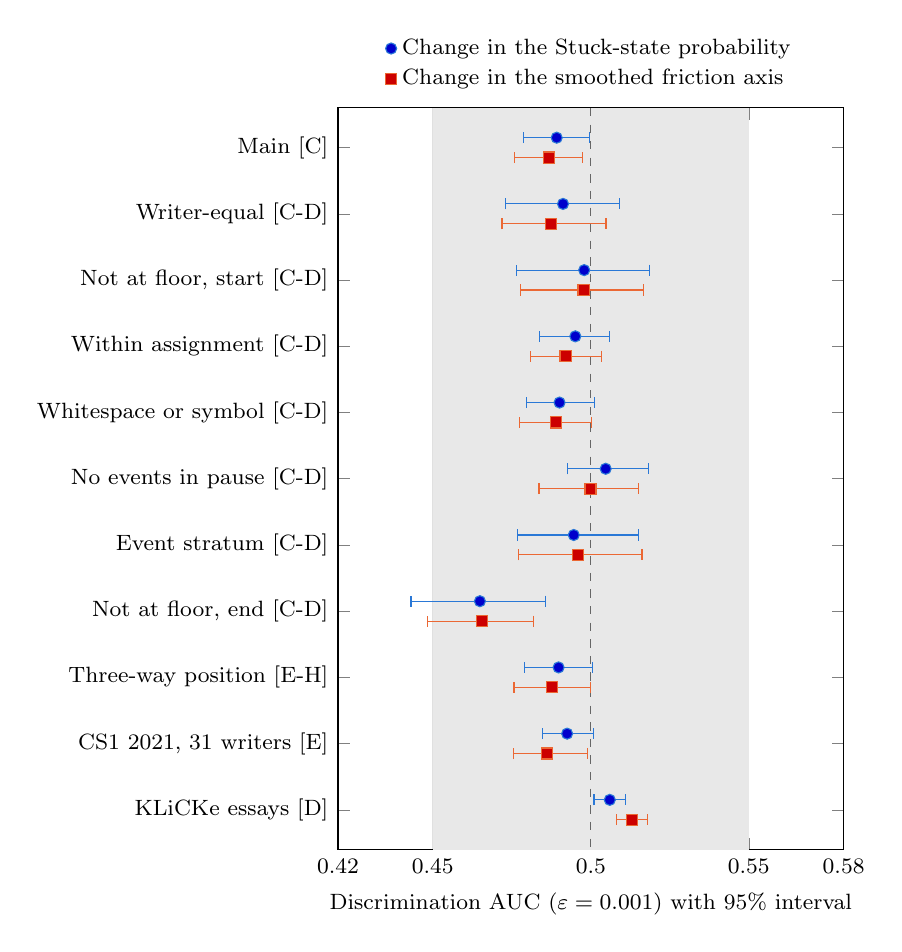
\begin{tikzpicture}
    \begin{axis}[
      width=0.66\linewidth, height=11cm,
      xmin=0.42, xmax=0.58, xtick={0.42,0.45,0.50,0.55,0.58},
      x tick label style={/pgf/number format/fixed, /pgf/number format/precision=2, font=\footnotesize},
      xlabel={Discrimination AUC ($\varepsilon = 0.001$) with 95\% interval}, label style={font=\footnotesize},
      ytick={1,...,11}, y dir=reverse, ymin=0.4, ymax=11.6,
      yticklabels={{Main [C]}, {Writer-equal [C-D]}, {Not at floor, start [C-D]}, {Within assignment [C-D]},
        {Whitespace or symbol [C-D]}, {No events in pause [C-D]}, {Event stratum [C-D]}, {Not at floor, end [C-D]},
        {Three-way position [E-H]}, {CS1 2021, 31 writers [E]}, {KLiCKe essays [D]}},
      y tick label style={font=\footnotesize, align=right},
      legend style={font=\footnotesize, draw=none, at={(0.5,1.01)}, anchor=south, legend columns=1}, legend cell align=left,
      xmajorgrids, major grid style={black!12},
    ]
      \fill[figband] (axis cs:0.45,0.4) rectangle (axis cs:0.55,11.6);
      \draw[black!60, dashed] (axis cs:0.5,0.4) -- (axis cs:0.5,11.6);
      \addplot+[only marks, mark=*, color=figc1, error bars/.cd, x dir=both, x explicit]
        coordinates {
          (0.4892,0.85) -= (0.0105,0) += (0.0103,0)
          (0.4912,1.85) -= (0.0182,0) += (0.0178,0)
          (0.4979,2.85) -= (0.0215,0) += (0.0206,0)
          (0.4951,3.85) -= (0.0113,0) += (0.0107,0)
          (0.4901,4.85) -= (0.0104,0) += (0.0111,0)
          (0.5047,5.85) -= (0.0121,0) += (0.0135,0)
          (0.4946,6.85) -= (0.0177,0) += (0.0204,0)
          (0.4649,7.85) -= (0.0218,0) += (0.0207,0)
          (0.4898,8.85) -= (0.0108,0) += (0.0108,0)
          (0.4925,9.85) -= (0.0079,0) += (0.0083,0)
          (0.506,10.85) -= (0.005,0) += (0.005,0)
        };
      \addlegendentry{Change in the Stuck-state probability}
      \addplot+[only marks, mark=square*, color=figc2, error bars/.cd, x dir=both, x explicit]
        coordinates {
          (0.4867,1.15) -= (0.0109,0) += (0.0108,0)
          (0.4875,2.15) -= (0.0156,0) += (0.0173,0)
          (0.4977,3.15) -= (0.0200,0) += (0.0190,0)
          (0.4920,4.15) -= (0.0112,0) += (0.0115,0)
          (0.4890,5.15) -= (0.0115,0) += (0.0113,0)
          (0.4999,6.15) -= (0.0163,0) += (0.0151,0)
          (0.4960,7.15) -= (0.0189,0) += (0.0202,0)
          (0.4656,8.15) -= (0.0173,0) += (0.0162,0)
          (0.4877,9.15) -= (0.0120,0) += (0.0122,0)
          (0.4861,10.15) -= (0.0107,0) += (0.0129,0)
          (0.513,11.15) -= (0.005,0) += (0.005,0)
        };
      \addlegendentry{Change in the smoothed friction axis}
    \end{axis}
  \end{tikzpicture}
  \caption{Discrimination AUC of the main analysis, the sensitivity analyses and the exploration, with the equivalence
  band shaded. Labels give the status of each analysis (Table~\ref{tab:status}). Values with $\varepsilon = 0$ are
  in Table~\ref{tab:main} and Appendix~\ref{app:sensitivity}.}
  \label{fig:forest}
\end{figure}

The levels of the signals at $u$ discriminated slightly more than their changes, and also stayed inside the band:
0.524 (0.510--0.537) for the Stuck-state probability and 0.521 (0.508--0.535) for the friction axis [C-D]. In the essay
data seen before the study, the same statistic gave 0.506 (0.501--0.511) and 0.513 (0.508--0.518) for the changes and
0.569 and 0.580 for the levels [D]. With the 90th percentile of each writer's controls as the threshold, 10.3\% of stall
run-ups exceeded it on the Stuck-state probability and 9.3\% on the friction axis, against 9.6\% of controls [C-D] (the control rate is about 10\% by construction); the differences, +0.7 and
$-0.3$ points, had writer-resampled intervals of $-0.2$ to 1.6 and $-1.2$ to 0.5 points [E-H], both including 0. These
are rates in the selected set of stalls and controls, not the performance of a trigger with a threshold set
independently and run continuously.

\subsection{On the same pairs, learners on simple quantities of preceding typing exceeded the two changes outside the registration}
\label{sec:res-learners}

This comparison sets the estimator's signals beside standard quantities judged against the same partner. In the
registered description [C-D], learners on 18 quantities of the preceding typing (Section~\ref{sec:design}) passed their
gate on the holdout: with a known difference added to one quantity so that its own AUC was 0.580, both recovered an
interval with a lower bound above 0.55. Logistic regression reached 0.567 (0.5497--0.578) and gradient boosting 0.540
(0.525--0.558), with intervals from 200 resamples of writers; both intervals cross 0.55, so the learners neither
established nor excluded an AUC above 0.55, for logistic regression only at the resolution of 200 resamples. Applied to
unmatched windows, the same learners gave 0.529 (0.512--0.546) and 0.526 (0.511--0.541), so they did not exceed a lower
bound of 0.55 there either (Appendix~\ref{app:learners}).

Outside the registration [E-H], with the learners' statistic ($\varepsilon = 0$) and over their 200 resamples (which
reproduced the registered values exactly), logistic regression exceeded the two 30-second changes by 0.078 (95\% interval
0.057--0.093) and 0.081 (0.057--0.097), and the levels of the signals at $u$ by 0.042 (0.019--0.059) and 0.046
(0.021--0.064); gradient boosting exceeded the changes by 0.051 and 0.054 but not clearly the levels. The learners can
use either direction of a quantity, whereas each signal was ranked in a fixed direction; read without direction (the
larger of the AUC and one minus it for the signals), logistic regression exceeded the changes by 0.057 (0.032--0.070)
and 0.054 (0.033--0.066), and gradient boosting by 0.030 and 0.027 (lower ends 0.009 and 0.008). Taken alone, the
quantities closest to the learners were levels over the 30~s before $u$: stalls were preceded by fewer key presses (AUC
0.446) and fewer characters per minute (0.443), whereas every 30-second change among the 18 quantities lay between
0.492 and 0.508; we did not decompose the learners. Because condition A becomes true earlier after less net production
(Appendix~\ref{app:definitions}), the stall definition could itself tie stalls to less preceding typing. Among the 3,426
stalls whose onset it did not bring forward ($s - u = 30$~s), the AUC of the number of key presses was 0.467 (0.393
among the 1,057 with $s - u < 30$~s; the other 71 stalls, with $s - u > 30$~s, are in neither group), and the
comparison, rerun on these stalls with the learners refitted, gave logistic regression 0.550 (0.527--0.562); read
without direction, it exceeded the two changes by 0.037 (0.012--0.056) and 0.031 (0.009--0.044), while gradient
boosting did not clearly exceed them (0.016 and 0.010, intervals including 0). By the reading committed before this
computation, the difference is therefore not explained by the definition of a stall alone, although it is smaller
there (Appendix~\ref{app:learners}).

\subsection{The main sensitivity analyses were also equivalent}
\label{sec:res-sens}

Of the preregistered sensitivity analyses, four bear on how the main result should be read [C-D]
(Figure~\ref{fig:forest}). The Stuck-state probability is mostly at the floor of the estimate: 61\% of stalls and 65\%
of controls had a probability below 0.02 at $u$, and none was above 0.98. Keeping only the pairs whose stall and control were both off the floor
at the start of the window, $u - 30$~s, left 2,090 stalls and gave 0.498 for both signals, equivalent under both
tolerances. Drawing controls only within the same assignment gave 0.495 and 0.492; matching on whether the character at
$u$ is whitespace or a symbol, instead of a newline, gave 0.490 and 0.489. Extending the stratum window to the end of
the pause, which removes stalls with a run, paste or switch inside the pause, left 2,427 stalls and gave 0.505
(0.493--0.518) and 0.500 (0.484--0.515). All four were equivalent for both signals and both tolerances. Selecting
off-floor pairs at the end point $u$ instead gave about 0.465 with intervals crossing 0.45 (undecidable on the lower
side); that version selects on the level reached at $u$ and thus on the change itself, which is why the start-point
version was registered as the main one. The event stratum gave 0.495 and 0.496 (effective writers 35.7). The remaining
sensitivity analyses, all equivalent, and the spread over the seed of the control draw are in
Appendix~\ref{app:sensitivity}.

\subsection{The unmatched comparison did not show a rise beyond the band}

In the secondary comparison of windows within writers, the unmatched AUC was 0.497 (0.491--0.503) for the Stuck-state
probability and 0.494 (0.489--0.4997) for the friction axis [C-D]. The registered condition, a lower bound above 0.55,
was not met, so we report only the equivalence in the matched comparison and do not contrast the two
(Appendix~\ref{app:unmatched}).

\subsection{Outside the registration, the estimator barely registered changes of the observed size}
\label{sec:res-bounds}

Three explorations outside the registration, each with conditions committed before it was computed, bound how the
equivalence can be read. They do not enter the decision.

\paragraph{Positive control of the estimator [E].} On the 319 seen writers, we rebuilt the estimate rows after changing
the key presses in the 30~s before every stall's $u$, keeping the stalls, controls and draws fixed. The intervals
between key presses were multiplied by $k$ (keeping the press at $u$), or a backspace and a retyped key were inserted
into a share $r$ of the intervals (Table~\ref{tab:poscontrol}). Because the estimator carries its state forward, the change also altered 34--47\% of the drawn
controls at the larger sizes, so we also report a version that keeps the controls at their unchanged values. The
observed difference was small and ran the other way: in the 30~s before $u$, the median of the mean interval between
presses was 598~ms for stalls and 605~ms for controls (a ratio of about 1.01), and the median share of backspaces 0.091
and 0.100. The injected changes ran opposite to this difference, and changes in its direction were not made. Slowing the run-up
by 2--10\%, more than the difference, hardly moved the AUC: 0.492--0.499. With controls
fixed, the friction axis left the band only when the intervals were doubled or half of them received a correction; the
Stuck-state probability did not leave the band even when the intervals were tripled (0.553, an interval crossing 0.55)
and fell when corrections were added. The levels of the signals at $u$, 0.526 and 0.527 unchanged, left the band at
smaller changes than their 30-second changes (Table~\ref{tab:poscontrol-all}).

\begin{table}
  \caption{Positive control on the seen CS1 writers [E]: discrimination AUC ($\varepsilon = 0.001$) after changing the key
  presses in the 30~s before each stall's $u$, with the controls re-estimated or kept at their unchanged values. Values
  whose 95\% interval lies outside the band are in bold; the half-width of the intervals was 0.007--0.008. Selected
  sizes; all sizes and the levels are in Table~\ref{tab:poscontrol-all}.}
  \label{tab:poscontrol}
  \centering\small
  \begin{tabular}{l cc cc}
    \toprule
    & \multicolumn{2}{c}{Controls re-estimated} & \multicolumn{2}{c}{Controls fixed} \\
    Change & $\Delta p_{\mathrm{stuck}}$ & $\Delta x$ & $\Delta p_{\mathrm{stuck}}$ & $\Delta x$ \\
    \midrule
    None & 0.492 & 0.490 & 0.492 & 0.490 \\
    Intervals $\times 1.02$ & 0.493 & 0.493 & 0.493 & 0.492 \\
    Intervals $\times 1.1$ & 0.499 & 0.498 & 0.498 & 0.496 \\
    Intervals $\times 1.5$ & 0.518 & 0.524 & 0.515 & 0.523 \\
    Intervals $\times 2$ & 0.537 & \textbf{0.564} & 0.532 & \textbf{0.564} \\
    Intervals $\times 3$ & \textbf{0.562} & \textbf{0.627} & 0.553 & \textbf{0.626} \\
    Corrections, $r = 0.05$ & 0.496 & 0.512 & 0.490 & 0.509 \\
    Corrections, $r = 0.25$ & 0.500 & \textbf{0.562} & 0.480 & 0.557 \\
    Corrections, $r = 0.5$ & 0.495 & \textbf{0.563} & 0.469 & \textbf{0.558} \\
    \bottomrule
  \end{tabular}
\end{table}

\paragraph{Scaled inputs at their floor or ceiling [E-H].} On the holdout's main stratum we replayed every assignment
again to read the estimator's window quantities. At
$u$, each of the four scaled inputs was pinned at 0 or 1 in a large share of stalls: the flight time at its floor in
72\% (at its ceiling in 10\%), the share of pauses after deletions in 83\% (9\%), the correction ratio in 32\% (35\%) and
the number of pauses in 54\% (17\%); the number of pauses moved from its ceiling at $u - 30$~s (51\%) to its floor at
$u$. The 30-second change was exactly zero in 63\% of stalls for the flight time and 73\% for the share of pauses after
deletions. Controls were alike (Table~\ref{tab:phi}). Part of the equivalence may therefore come from the floor and
ceiling of the scaling on this input.

\paragraph{Later-pause controls [E-H].} A trigger that fires after a pause has lasted $x$ seconds compares stalls with
pauses that outlasted $x$. Restricting the controls in the holdout to pauses of at least 5~s or 10~s gave 0.491 and 0.491,
and 0.494 and 0.497, all inside the band (effective writers 49.8 and 48.6).

\subsection{In the exploration outside the registration, the discrimination AUC also stayed inside the band}
\label{sec:res-explore}

After the confirmation we applied the same procedure, with conditions committed before each computation, to other data
(Table~\ref{tab:explore}). In the 31 seen writers of the 2021 CS1 edition, all four combinations were inside the band
[E]. Matching stalls and controls on three positions at once (after a newline, after a token boundary, within a token)
in the holdout gave 0.490 and 0.488 [E-H]; stalls were slightly more frequent after a token boundary than controls (53.9\%
against 50.9\%). The procedure also ran on the full essay corpus and on the seen co-writing data (Appendix~\ref{app:explore}).

\begin{table}
  \caption{Exploration outside the registration: discrimination AUC of the 30-second change ($\varepsilon = 0.001$; the
  value with $\varepsilon = 0$ differs by at most 0.001).}
  \label{tab:explore}
  \centering\small
  \begin{tabularx}{\linewidth}{>{\raggedright\arraybackslash}X l c c}
    \toprule
    Data & Status & $\Delta p_{\mathrm{stuck}}$ & $\Delta x$ \\
    \midrule
    CS1 2021 edition, 31 seen writers & [E] & 0.493 (0.485--0.501) & 0.486 (0.475--0.499) \\
    CS1 2019 holdout, three-way position & [E-H] & 0.490 (0.479--0.5006) & 0.488 (0.476--0.4999) \\
    \bottomrule
  \end{tabularx}
\end{table}

\section{Discussion}
\label{sec:discussion}

In the CS1 holdout (139 students), the discrimination AUC of the 30-second change at $u$, in the matched comparison, fell
within the band $[0.45, 0.55]$ set in advance. Equivalence here
means that each signal, used alone as a ranking score, separated stall run-ups from matched control run-ups no better
than the band allows, on average over the pairs weighted within writers. It does not mean that typing does not change
before a stall, that stalls and controls did not both change, that a combination of signals could not separate them, or
that the signals are uninformative for every writer.

For research and practice that builds triggers for help from keystrokes, the result concerns one quantity: the change of
this estimator's two signals over the 30~s up to the last character input before a stall. It does not address what
happens later in the pause, where both signals rose (Section~\ref{sec:data}), nor a firing rule that uses the length of
the pause itself. The registered reading for a trigger is the threshold table: at each writer's 90th percentile of
controls, 10.3\% and 9.3\% of stall run-ups exceeded the threshold, against 9.6\% of controls (Section~\ref{sec:res-main}).
A conversion made after the band was set, on seen writers, under a model that shifts the stall values by a constant
and fires when a pause in the no-event stratum reaches 2~s (Appendix~\ref{app:threshold}), puts the share of firings
on pauses that become stalls at 8.2--8.9\% at an AUC of 0.50 and 8.9--10.0\% at 0.55, a rise of 0.1--1.8 points. The
low base rate sets most of this: even at 0.70 the share was 12.9--18.4\%, and a trigger that waits longer in the pause
meets a higher base rate. In that sense the 30-second change gave no basis for a trigger on this input; a trigger whose
threshold is fixed independently and whose hit rate and false alarms per hour are measured could behave differently. Those who plan to use an estimator of the same type as a trigger can
check its run-up signal against a band set in advance \cite{lakens2017equivalence} on held-out writers
\cite{gardner2018evaluating}; our data do not show the harm of omitting the check.

\subsection{How far the instrument explains the equivalence}

The equivalence could reflect the instrument rather than the typing: the input was rebuilt from edit events with a
synthesised release, the coefficients were not estimated on these data, and the levels discriminated less in CS1 (0.524
and 0.521) than in the essays (0.569 and 0.580). The positive control shows that the estimator is not inert on this
input, but also that changes of the size observed between stalls and controls barely move its 30-second changes, and
that its Stuck-state probability does not register corrections as friction; many of its scaled inputs sat at their
floor or ceiling, so a small change often leaves them unchanged. The main intervals exclude differences larger than
about 0.025 from 0.5 (a description made after the data were seen), and at this resolution the instrument cannot show
whether the run-up differs by the observed amount. The learners point to a difference of another kind: stalls were
preceded by less typing, a level rather than a change, partly because of how a stall is defined, and the estimator's
30-second changes are not built to carry it. The result is therefore a
statement about this instrument on this input, not about the absence of differences in the typing before stalls.

\subsection{What was established and what remains possible}

What the registration establishes is limited to the statistic above being inside the band in the matched comparison,
including after removing stalls that contain events inside the pause. The weak response to small changes, the floor of
the scaled inputs and the level difference are explorations; they bound the reading but were not tested. Whether unmatched evaluation makes run-up rises look large
cannot be judged here: the unmatched comparison showed no rise, and in the learner description the matched comparison
was higher than the unmatched windows (Section~\ref{sec:res-learners}). Nor can the opposite reading, that matching
removed a real run-up difference \cite{mansournia2018case}, be supported or excluded. The result is consistent with the
parallel view of planning (Section~\ref{sec:intro}) but is not a test of it, because a serial view that allows planning
to start late in the run-up would predict the same, and the view concerns language boundaries in prose rather than long
stops in code. The direction slightly below 0.5 and its candidate causes are
discussed in Appendix~\ref{app:sensitivity}.

\subsection{Calibration and reporting}

The decision rule declared equivalence more often than its nominal level in one of its two versions
(Section~\ref{sec:design}), as is known for cluster-level inference with few or unequal clusters
\cite{cameron2008bootstrap,cameron2015practitioner,mackinnon2023cluster}; designs with few effective writers may
benefit from a similar calibration. In other fields, unmatched controls have made accuracy look
larger \cite{lijmer1999empirical,pepe2008pivotal}; stating what the comparison partner was matched on lets readers judge
a run-up signal, although our data do not show an effect of the way of matching.

\subsection{Materials}

No new data were collected; the analyses used de-identified public datasets under the terms set by their authors. We
release the preregistration, the deviation, the start records and the results registration (all public on the Open
Science Framework), and an archive (version 0.1.0, \url{https://doi.org/10.5281/zenodo.24014043}) with the estimator and
the replay tool cut out at the version used, the code of the evaluation, the explorations and the conversion of the
public data, the seed and the computational environment, the manifest of the verified files, the conditions committed
before each computation (in Japanese, with an English summary) and the aggregate results. On every call that the
paper's pipelines made on the seen CS1 2019, essay and co-writing data, the released estimator returned output
byte-identical to the build used for the analysis; the calls of the 2021 data and of the positive control were not
compared, and rerunning the comparison needs that build, which is not distributed. The archive gives the steps to obtain
the public data and to rerun the confirmation on the holdout; run with the released estimator, they reproduced the
released result byte for byte. The order of the records can be checked from outside only
through the timestamps of the registrations; the commit times of the conditions come from the authors' private history,
and six files of the manifest are documents of that history, three of which (the preregistration text and its English
check) are attached to the registration. The CS1 files are released by their authors on request, and we agreed to publish
only aggregate values, so neither the data nor the per-pause estimate rows are redistributed. The list of holdout writers
will be added if the authors of the data agree; otherwise its SHA-256 and the procedure that drew it are given.

\section{Limitations}
\label{sec:limitations}

The confirmation used one introductory programming dataset and one estimator with hand-set coefficients. The
equivalence concerns this estimator on this input, the no-event stratum, stalls and controls with condition A false at
$u$, and the discrimination AUC of each signal alone, averaged over pairs; it says nothing about small differences inside
the band, combinations of signals or individual writers.

The registered positive control applied only to the learners. The estimator's positive control was added afterwards on
seen writers and injected changes only opposite to the observed difference; with the pinned scaled inputs, the
equivalence cannot be told apart from a weak response of the instrument to small changes on this input.

The band was set wide after we had seen the essay and co-writing data and was not derived from a conversion;
it is not justified as a practical boundary and is wider than the field's precedent of 0.01 for differences between two
models \cite{gardner2018evaluating}. That precedent compares a different quantity, but applied to our statistic, the
distance of the point estimates from 0.5 (about 0.011 to 0.013) would not count as equivalent.

The confirmation was made after a leak had shown that, under an older definition, the AUC on seen writers lay inside
the band. The false-equivalence rate was at most 5.2\% in
the version with replacement, about that of an ordinary two one-sided tests procedure at one-sided 5\%, and at most 1.4\%
in the version without, among the configurations examined; it is not an
upper bound over the whole null, it does not account for selecting the maximum, and its mechanism was not tested. The
decision rule was not changed, and the preregistration requires this qualification in the main sentence wherever it
appears, including the abstract.

The Stuck-state probability is mostly at the floor (61\% of stalls, 65\% of controls), so claims about run-up change
rely on the friction axis and on the pairs not at the floor.

A stall is a stop in character production, not a judgement of being stuck, and it was not checked against evidence
beyond keystrokes such as speech or self-report; nor did we check how often stalls coincide with moments at which help
would be useful. In the holdout's main stratum, 47\% of stalls contained a run of the program, a paste or a switch
inside the pause, and stops of 30~s or more can include time spent outside the assignment, so many stalls may be ordinary
breaks in work rather than moments at which help is needed. Pauses can contain non-character key presses. The personalised threshold decides when a stall is
recognised; its 0.99 quantile was inherited, and the 30~s and 2~s limits are fixed. The comparison with the learners and
the lengths of stalls were computed on the holdout after it had been opened.

The input was built from edit events with a release 100~ms after each press, so flight times and the meaning of
corrections, bursts and pauses after deletions may differ from writing with recorded releases
(Table~\ref{tab:mapping}).

Matching was on writer, boundary type (newline) and stratum; other factors, such as the phase of the assignment or the amount of
preceding typing, were not matched, and only controls are excluded by proximity to a later onset. Because condition A
becomes true earlier after less net production, the definition of a stall itself ties stalls to less preceding typing.

The per-pause estimate rows are not shared, under the terms agreed for the CS1 files; the holdout values can be
reproduced from outside only by obtaining the files and rerunning the released code and estimator. The learners'
intervals come from 200 resamples of writers. Nothing is claimed about Japanese, input method editors, natural work or other populations.

\section{Conclusion}
\label{sec:conclusion}

In the CS1 holdout (139 students), the discrimination AUC of the 30-second change at $u$ of the estimator's two signals,
in the matched comparison, fell within the band $[0.45, 0.55]$ set in advance, and its intervals excluded differences
larger than about 0.025 from 0.5 (Section~\ref{sec:limitations} qualifies the error rate). Changes of the observed size
barely moved these signals, and simple quantities ranked the same pairs higher through the amount of preceding typing.
Under a conversion made after the band was set, a difference at the band's edge would change the share of trigger firings
that fall on stalls by about one point, so on this input the 30-second change of this estimator gave no basis for a
trigger before stalls in character production.

\section*{Declaration of Generative AI Software Tools in the Writing Process}

% The wording below follows the journal's required sentence.
During the preparation of this work, the author used Claude (Anthropic) in all sections and in the supplementary
material in order to draft the text and the tables from the author's analysis records, to write the analysis scripts
under conditions fixed in advance, to search the literature, and to check the numbers against the result files. After
using this tool, the author reviewed and edited the content as needed and takes full responsibility for the content of
the publication.


\bibliographystyle{acmtrans}
\bibliography{references}

\appendix
% Supplementary material, placed after the references as the journal's instructions ask. Sections S1 to S10 are
% referred to from the main text by their labels.
\renewcommand{\thesection}{S\arabic{section}}
\setcounter{section}{0}

\section{Registration, deviation and the order of the records}
\label{app:prereg}

\paragraph{Registrations.} All registrations are Open-Ended Registrations of one project on the Open Science Framework
and are public. The preregistration (English version governing; a Japanese version is attached) was registered at
2026-11-05 21:56:19 UTC (\url{https://osf.io/mrkxt}); its field holds the SHA-256 of the manifest of the verified files
(scripts, conversion, holdout procedure, environment, stall definition and the two language versions of the document).
The deviation was registered with the new manifest (\url{https://osf.io/fqgcp}); the second start record is at
\url{https://osf.io/ajg2x}, and the results and their provenance at \url{https://osf.io/uj6cy}, registered at
2026-11-06 02:48:02 UTC.

\paragraph{Two-stage procedure.} Stage 1 verifies the manifest, the inputs, the holdout list, the replay tool and the
environment against the values passed to it, writes a start record and stops without computing; the start record is
then registered. Stage 2 takes the SHA-256 of the registered start record, repeats the verification, commits a record
of the start of computation and only then computes. The confirmation script refuses to run unless both records are
committed and agree. A completed run cannot be repeated.

\paragraph{Order of events (UTC).} The holdout list had been drawn before any analysis of the CS1 data; the conditions
of the first analysis of these data (committed on 2026-11-03 at 23:46) skipped the listed writers and required a check
that none of them entered its aggregates. On 2026-11-05 and 2026-11-06, the registrations (OSF) and the commits of the
local repository (git) were, in order:

\begin{center}\footnotesize
\begin{tabular}{l l l}
  \toprule
  Time & Record & Event \\
  \midrule
  21:56:19 & OSF & preregistration registered (\url{https://osf.io/mrkxt}) \\
  21:58:55 & git & first start record written and committed \\
  23:16:27 & OSF & first start record registered (\url{https://osf.io/hfvy7}) \\
  23:17:58 & git & first computation started (stopped at 23:24:44 in the conversion check) \\
  01:23:42 & OSF & deviation registered (\url{https://osf.io/fqgcp}) \\
  01:25:11 & git & outputs of the stopped run moved aside \\
  01:25:12 & git & second start record written and committed \\
  01:26:12 & OSF & second start record registered (\url{https://osf.io/ajg2x}) \\
  01:27:32 & git & second computation started \\
  02:22:48 & git & completed run committed \\
  02:48:02 & OSF & results and provenance registered (\url{https://osf.io/uj6cy}) \\
  \bottomrule
\end{tabular}
\end{center}

The first computation stopped because the registered check ``the number of writers read equals the number of writers
in the holdout list'' gave 145 of 146. No statistic had been computed. The cause was a holdout writer whose only raw
row was a checkpoint and who therefore had no assignment; this writer would have been excluded in any case. At the
researcher's decision the check was replaced by one that requires every writer read to be in the list, every writer not
read to have no rows that create an assignment under the same mapping, and the two counts to sum to 146 (negative
controls: removing a writer read, or adding a writer outside the list, both fail). Nothing else changed. In the local
history there were two start records, one interruption, one move-aside, two computation starts and one completed run.

\paragraph{Archive and provenance.} The archive holds the seed and the computational environment and the manifest of the
verified files besides the items named in the main text. The released estimator's output matched the analysis build
byte for byte on every call made on the seen CS1 2019, essay and co-writing data; the calls of the 2021 data and of the
positive control were not compared, and the analysis build is not distributed. A first run of that comparison on CS1 with seven parallel jobs, when the free disk space was near zero, logged
differing output in 9 of the 1,079 \texttt{--features} calls and differing exit codes in 8 (one a crash of the
analysis build); their cause was not
established, and the rerun with four jobs, on which the statement rests, had none. Run with the released estimator on the
authors' machine (macOS arm64), the archive's steps for the holdout reproduced the released result byte for byte; the
explorations are released as scripts without such a rerun check. The order of the records can be checked from outside
only through the timestamps of the registrations; the commit times of the conditions come from the authors' private
history, and six files of the manifest are documents of that history, three of which (the preregistration in Japanese
and in English, and the check of the English version) are attached to the registration. The list of holdout writers will
be added if the authors of the data agree.

\paragraph{Wording.} The registration attaches the false-equivalence qualification to the main sentence and keeps it in
the abstract; the paper gives it in full in the abstract, the conclusion, the calibration and the limitations, and
refers to the limitations elsewhere. The registration's main sentence speaks of ``the rise in the run-up in the matched comparison'';
the paper names the same statistic ``the discrimination AUC of the 30-second change''. The registration's rule for the
second sentence applied because the not-at-floor sensitivity analysis selected at the start point was equivalent for
the Stuck-state probability under both tolerances. Intervals in the OSF summary have three digits; in the paper, an end
of an interval that touches 0.45, 0.5 or 0.55 at three digits is given with four. The registration labels the
confirmatory test H1, the unmatched comparison H2 and the learner description H3. The registration says the band was set
``conservatively''; the paper says ``wide'', because a wide band makes equivalence easier to declare. The registration
says the confirmation ``is not written as a test of a prediction that could fail''; the abstract and introduction say
so in those terms. The registration says the estimator ``was applied with the writing coefficients as they are (not
adapted to individuals or to programming)''; the reference values for direct input had been adjusted for code-like
input when they were introduced for alphanumeric input, before this study, and were kept unchanged
(Appendix~\ref{app:coefficients}).

\paragraph{History of the learner analysis.} In the drafts of the registration the learner analysis was confirmatory,
with a positive control that required the learners to exceed 0.55 on unmatched windows. On seen writers this control
did not pass for either learner, so the gate was replaced by the recovery of a known embedded difference and the
analysis was downgraded to a description, all before freezing. The unmatched-window result is still reported.

\paragraph{What was known before the confirmation.} The matched comparison had been computed on the essay and co-writing
data before the registration was written, and the band was set afterwards. On the 319 seen CS1 writers, an output of a
pre-freeze computation leaked the constants used to shift provisional signals, which revealed that under that
computation's older definition the AUC was slightly above 0.50 and below 0.55. Which rules were fixed before and after
that leak is tabulated in the registration (its Appendix B).

\section{Definitions}
\label{app:definitions}

\paragraph{Statistic.} For signal $z$, writer $i$, cell $c$ (boundary type and stratum), stalls $S_{ic}$ and the set
$K_{ic}$ of distinct controls drawn for them,
\[
\mathrm{AUC} = \frac{\sum_{i,c} \sum_{a \in S_{ic}} \sum_{b \in K_{ic}} \phi_\varepsilon(z_a - z_b)}
{\sum_{i,c} |S_{ic}|\,|K_{ic}|}, \qquad
\phi_\varepsilon(d) = \begin{cases} 1 & d \ge \varepsilon \\ 0.5 & |d| < \varepsilon \\ 0 & d \le -\varepsilon
\end{cases}
\]
with $\phi_0(d) = 1, 0.5, 0$ for $d > 0$, $d = 0$, $d < 0$. The signal at $t$ is the latest estimate row at or before $t$
minus the latest row at or before $t - 30$~s; no maximum gap between $t$ and the row was set. In an audit after the
confirmation [E-H], the two rows lay in different observation segments, more than 2~s before their nominal times, or
outside 28--32~s apart for 70 of the 4,554 stalls (1.5\%) and 195 of the 18,689 controls (1.0\%) of the main stratum
(median lag 0.5~s, largest 6.8~s; span 30~s at the median and 99th percentile); without them the point estimates were
0.491 and 0.487 ($\varepsilon = 0.001$), against 0.489 and 0.487 with them. Stalls can arise only once $\theta$ is
defined, but controls were not required to have $\theta$ defined at $u$; it was undefined for 172 of the 18,689 controls
(0.9\%) and 1 stall, and restricting both to $\theta$ defined at $u$ gave 0.489 and 0.487 [E-H]. The decision is the conjunction over two
signals and two tolerances.

\paragraph{Missing values and exclusions.} A stall or control without an estimate row at or before $u$ or $u - 30$~s, or
with a non-numeric value, is dropped; a stall without any control is dropped. In the holdout's main analysis no stall
lacked a signal and 3 stalls had no control. Writers with less than 10 minutes of observation (5 in the holdout) and
assignments beyond the time span of the replay tool (none) are excluded.

\paragraph{Temporal boundaries.} The estimate rows are computed forward in time, so the signals at $u$ use only key
presses up to $u$. $\theta$ uses the intervals so far in the assignment and fixes only the onset. The learners' imputation
and scaling are fitted within the training folds, which are formed by writer.

\paragraph{Estimator.} Version 0.5.0 of the estimator was used with its writing configuration and without individual
calibration; the replay tool has SHA-256 \texttt{\seqsplit{26cae610383fb6de01651cc904895efa72a691c3dd1e27689a14a4ca51c33bb3}}. The
transition and emission matrices and the weights of the two axes were set by hand from the literature and informal
tuning. For direct (non-IME) input, the reference values against which the five quantities are scaled were set by hand
from population medians of typing \cite{dhakal2018typing}, adjusted for code-like input; they were introduced for
alphanumeric input and later kept, unchanged, in the writing configuration. None of the coefficients were estimated
from the data analysed here. The friction axis is smoothed exponentially with coefficient 0.3.

\paragraph{Mapping of edit events.} The rules of Section~\ref{sec:data} were fixed in an earlier analysis of the CS1
data, before this study. Keystrokes are ordered by client timestamp and, within ties, by event identifier. The release is
placed 100~ms after the press and cut 1~ms before the next press, so the estimator's flight time is the inter-keystroke
interval minus 100~ms when the interval exceeds 100~ms, 1~ms for shorter intervals and 0 for simultaneous presses, a
definition that differs from that of recorded releases in writing data. Every insertion with a recorded key was a single
character. In the holdout as a whole, the share of estimate rows with a Stuck-state probability below 0.02 ranged from
26\% to 62\% per writer between the 10th and 90th percentiles, and the standard deviation of the 30-second change over
all estimate rows was 0.270 for the Stuck-state probability and 0.187 for the friction axis [E-H].

\begin{table}[h]
  \caption{How the edit rows of the holdout writers were mapped to the estimator's input (exploration on the holdout,
  counted after the confirmatory run; 1,490,503 edit rows). Shares of characters are of all inserted characters.}
  \label{tab:mapping}
  \centering\small
  \begin{tabularx}{\linewidth}{>{\raggedright\arraybackslash}X >{\raggedright\arraybackslash}p{2.9cm} r r}
    \toprule
    Edit row & Becomes & Rows & Characters \\
    \midrule
    Insertion of one character, key recorded & key press of its kind & 78.2\% & 46.3\% \\
    Deletion of one character, key recorded & backspace & 19.5\% & -- \\
    Deletion of two or more characters, key recorded & backspace (one press) & 0.37\% & -- \\
    Undo or redo & non-text key press (key recorded) or event & 0.46\% & -- \\
    Insertion of whitespace only, no key (automatic indentation) & event & 1.0\% & 4.6\% \\
    Paste & event & 0.37\% & 49.0\% \\
    Other (cut, drag, checkpoint, other insertions without key) & event or nothing & 0.11\% & $<$0.1\% \\
    \bottomrule
  \end{tabularx}
\end{table}

\paragraph{Stall definition.} Condition A is evaluated at the key press times, at those times plus 30~s and at $s +
\theta$. $\theta$ is the nearest-rank 0.99 quantile of intervals between adjacent key presses of any kind within the
same observation segment, accumulated over segments in the assignment, and undefined below 100 intervals. Observation
segments break where 1~Hz estimate rows are more than 2~s apart, after the replay tool trims rows without input before
gaps of 60~s or more and across gaps of 30 minutes or more. In the seen 2019 writers, $\theta$ at the end of an
assignment had a median of 27.7~s (quartiles 20.8--36.8~s; 316 writers in the earlier analysis of these data) [D].
Edges of observation [E-H]: of 9,133 distinct $u$ of onsets in the holdout, 22 had no later character input in the
assignment and 51 had the next one in a later work block. A pause with no later character input is taken to end at the last key press of the assignment,
so such a stall is kept only if that press comes at least 30~s after $u$; a pause whose next character input lies in a
later work block ends at that input. When several onsets share the same $u$, only the first is considered, and it is
dropped, not replaced, if it fails a condition. $\theta$ is its value at $s$, from the intervals up to $s$. Inside the pause, in the holdout's main stratum, 47\% of stalls contained a run of the program, a paste or a switch,
against 6\% of controls; 52\% of stalls and 69\% of controls contained no key press of any kind, and the 90th percentile
of key presses inside the pause was 13 for stalls and 5 for controls. The onset came a median of 48.5~s after $u$ (10th and 90th percentiles 35.2 and 77.6~s; mean 247~s, because a few
onsets come long after the last character input), and the next character input a median of 97.2~s after $u$ (mean
428~s; 78.6\% of stalls lasted 60~s or more). The 338 seen writers with an assignment had 1,078
assignments, and the 319 kept writers 1,042.

\section{Coefficients of the estimator}
\label{app:coefficients}

All values below were set by hand (version 0.5.0); none were estimated from the data analysed here. They are taken
from the source of the estimator, which is released with the archive (Section~\ref{sec:discussion}).

\paragraph{Window quantities.} Every second, over the key events of the preceding 30~s: $f_1$, the median flight time
from a release to the next press, with flights of 2,000~ms or more dropped; $f_3$, the share of presses that are
backspaces; $f_4$, the mean burst length, a burst continuing while the flight is under 200~ms; $f_5$, the number of
intervals of 2,000~ms or more between adjacent presses; $f_6$, the share of backspaces followed by such an interval.
With the synthesised release (Section~\ref{sec:data}), a burst continues while inter-keystroke intervals are under
300~ms.

\paragraph{Scaling and axes.} Each quantity is scaled as $\varphi(f, \beta) = \min(1, \max(0, (f - \beta) / 2\beta))$
against a reference value $\beta$. For direct input, $\beta = 150$~ms ($f_1$), 0.06 ($f_3$), 5.0 ($f_4$), 2.0 ($f_5$)
and 0.08 ($f_6$). The friction axis is $x = 0.30\,\varphi_3 + 0.25\,\varphi_6 + 0.25\,\varphi_1 + 0.20\,\varphi_5$ and
the engagement axis $y = 0.40\,\varphi_4 + 0.35\,(1 - \varphi_1) + 0.25\,(1 - \varphi_5)$, both clipped to $[0, 1]$.

\paragraph{Smoothing and observations.} Both axes are smoothed exponentially, $s_t = \alpha\,r_t + (1 - \alpha)\,s_{t-1}$,
with $\alpha = 0.3$ while the window has input, and, during silence, $\alpha = 0.15$ below 15~s, 0.18 from 15 to 25~s and
0.25 from 25~s; the initial values are $(x, y) = (0.1, 0.8)$. The smoothed axes are binned as
$\lfloor 5 s \rfloor$ (capped at 4) into $5 \times 5$ observations, indexed $5\,b_x + b_y$; a 26th observation replaces
the binned one after 14 or more consecutive backspaces. During silence of 2~s or more with an empty window, the
quantities are replaced by a synthetic observation: $f_1 = 2{,}000$~ms, $f_4 = 0$, $f_5$ = silence in seconds / 2, and
$f_3, f_6$ carried over from the last typing window $v$ as $v + \min(1, (\mathrm{silence} - 2)/30)\,(1 - v)\,v$ (without
such a window, ramps of 10--50~s with floors of 0.15 and 0.20 from 10~s). When the window still holds input after 8~s
of silence, $f_3$ and $f_6$ are floored at $v \min(1, (\mathrm{silence} - 8)/30)$.

\paragraph{Hidden Markov model.} States are ordered Flow, Incubation, Stuck. Initial probabilities $(0.80, 0.15, 0.05)$.
Transition matrix (rows: from):
\[
\begin{pmatrix} 0.75 & 0.17 & 0.08 \\ 0.12 & 0.80 & 0.08 \\ 0.06 & 0.18 & 0.76 \end{pmatrix}.
\]
With $\pi_t$ the forward probabilities, $A$ the transition matrix and $e_j(o)$ the emission weight of state $j$ for
observation $o$, each update is $\pi_{t,j} \propto e_j(o_t) \sum_i \pi_{t-1,i} A_{ij}$, normalised over $j$; because
the emission weights are not normalised per state, this is a weighted filter rather than the forward algorithm of a
proper hidden Markov model. The reported probability is a further exponential smoothing of
them with coefficient 0.40 (0.60 at the backspace observation); the Stuck-state probability in this paper is that
reported value, and the friction axis is the smoothed $x$. Emission weights (rows $b_x = 0, \ldots, 4$ from low to high
friction, columns $b_y = 0, \ldots, 4$ from low to high engagement; the rows of the full matrix are not normalised):

\begin{center}\footnotesize
\setlength{\tabcolsep}{3pt}
\begin{tabular}{c ccccc c ccccc c ccccc}
  \toprule
  & \multicolumn{5}{c}{Flow} && \multicolumn{5}{c}{Incubation} && \multicolumn{5}{c}{Stuck} \\
  $b_x$ & 0 & 1 & 2 & 3 & 4 && 0 & 1 & 2 & 3 & 4 && 0 & 1 & 2 & 3 & 4 \\
  \midrule
  0 & .01 & .02 & .08 & .12 & .14 && .15 & .10 & .04 & .03 & .02 && .01 & .01 & .01 & .01 & .01 \\
  1 & .01 & .02 & .08 & .12 & .13 && .14 & .08 & .04 & .03 & .02 && .01 & .01 & .01 & .01 & .01 \\
  2 & .01 & .01 & .02 & .01 & .08 && .10 & .08 & .03 & .02 & .01 && .02 & .04 & .04 & .05 & .01 \\
  3 & .01 & .01 & .01 & .01 & .01 && .05 & .04 & .01 & .01 & .01 && .10 & .16 & .05 & .07 & .01 \\
  4 & .01 & .01 & .01 & .01 & .01 && .04 & .03 & .01 & .01 & .01 && .16 & .22 & .12 & .05 & .02 \\
  \midrule
  backspace & \multicolumn{5}{c}{.01} && \multicolumn{5}{c}{.01} && \multicolumn{5}{c}{.99} \\
  \bottomrule
\end{tabular}
\end{center}

\section{Sensitivity analyses and descriptions of the instrument}
\label{app:sensitivity}

Table~\ref{tab:sens} lists every preregistered sensitivity analysis of the matched comparison [C-D]. All results with
$\varepsilon = 0$ fell in the same category as those with $\varepsilon = 0.001$.

\begin{table}
  \caption{Sensitivity analyses of the matched comparison, CS1 holdout ($\varepsilon = 0.001$). Stalls are those of
  the no-event stratum; equiv. = equivalent, undec. = undecidable.}
  \label{tab:sens}
  \centering\footnotesize
  \setlength{\tabcolsep}{3pt}
  \begin{tabularx}{\linewidth}{>{\raggedright\arraybackslash}X r c c l}
    \toprule
    Analysis & Stalls & $\Delta p_{\mathrm{stuck}}$ & $\Delta x$ & Result \\
    \midrule
    Main & 4,554 & 0.489 (0.479--0.4995) & 0.487 (0.476--0.497) & equiv. \\
    Control pauses up to 10 s & 4,554 & 0.490 (0.480--0.5007) & 0.489 (0.478--0.499) & equiv. \\
    Control pauses up to 60 s & 4,554 & 0.490 (0.479--0.502) & 0.490 (0.478--0.502) & equiv. \\
    Boundary type: whitespace or symbol & 4,554 & 0.490 (0.480--0.501) & 0.489 (0.478--0.5003) & equiv. \\
    Stratum window to the end of the pause & 2,427 & 0.505 (0.493--0.518) & 0.500 (0.484--0.515) & equiv. \\
    No condition A on stalls & 4,915 & 0.497 (0.488--0.506) & 0.494 (0.484--0.504) & equiv. \\
    Condition A on neither side & 4,915 & 0.490 (0.480--0.4995) & 0.490 (0.478--0.5006) & equiv. \\
    Controls within the assignment & 4,553 & 0.495 (0.484--0.506) & 0.492 (0.481--0.503) & equiv. \\
    Writer-equal weights & 139 writers & 0.491 (0.473--0.509) & 0.488 (0.472--0.505) & equiv. \\
    Not at floor, start point $u - 30$ s & 2,090 & 0.498 (0.476--0.519) & 0.498 (0.478--0.517) & equiv. \\
    Not at floor, end point $u$ & 1,573 & 0.465 (0.443--0.486) & 0.466 (0.448--0.482) & undec. (lower) \\
    Signal change over 15 s & 4,554 & 0.491 (0.480--0.502) & 0.485 (0.473--0.496) & equiv. \\
    Signal change over 60 s & 4,553 & 0.496 (0.486--0.506) & 0.495 (0.485--0.505) & equiv. \\
    $\theta$ accumulated across assignments & 4,445 & 0.487 (0.477--0.498) & 0.487 (0.476--0.497) & equiv. \\
    Stall quantile $q = 0.995$ (warm-up 200) & 2,935 & 0.490 (0.476--0.503) & 0.487 (0.473--0.501) & equiv. \\
    Condition A window $W = 15$ s & 5,937 & 0.493 (0.483--0.503) & 0.490 (0.479--0.5005) & equiv. \\
    Condition A window $W = 60$ s & 2,976 & 0.494 (0.480--0.507) & 0.493 (0.479--0.508) & equiv. \\
    Event stratum (described) & 1,590 & 0.495 (0.477--0.515) & 0.496 (0.477--0.516) & equiv. \\
    \bottomrule
  \end{tabularx}
\end{table}

\begin{table}
  \caption{Positive control on the seen CS1 writers [E], all sizes run: discrimination AUC ($\varepsilon = 0.001$) of the
  30-second changes and of the levels at $u$, with the controls re-estimated or kept fixed. Bold: 95\% interval outside
  the band. Unchanged, the rebuilt rows matched the stored ones in all 1,042 assignments.}
  \label{tab:poscontrol-all}
  \centering\footnotesize
  \setlength{\tabcolsep}{3pt}
  \begin{tabular}{l cccc cccc}
    \toprule
    & \multicolumn{4}{c}{Controls re-estimated} & \multicolumn{4}{c}{Controls fixed} \\
    Change & $\Delta p_{\mathrm{stuck}}$ & $\Delta x$ & $p_{\mathrm{stuck}}$ & $x$ & $\Delta p_{\mathrm{stuck}}$ & $\Delta x$ & $p_{\mathrm{stuck}}$ & $x$ \\
    \midrule
    None & 0.492 & 0.490 & 0.526 & 0.527 & 0.492 & 0.490 & 0.526 & 0.527 \\
    Intervals $\times 1.02$ & 0.493 & 0.493 & 0.528 & 0.530 & 0.493 & 0.492 & 0.528 & 0.529 \\
    Intervals $\times 1.05$ & 0.495 & 0.495 & 0.529 & 0.531 & 0.494 & 0.493 & 0.528 & 0.530 \\
    Intervals $\times 1.1$ & 0.499 & 0.498 & 0.534 & 0.536 & 0.498 & 0.496 & 0.534 & 0.535 \\
    Intervals $\times 1.2$ & 0.503 & 0.503 & 0.540 & 0.543 & 0.502 & 0.502 & 0.540 & 0.543 \\
    Intervals $\times 1.5$ & 0.518 & 0.524 & 0.558 & \textbf{0.569} & 0.515 & 0.523 & \textbf{0.560} & \textbf{0.574} \\
    Intervals $\times 2$ & 0.537 & \textbf{0.564} & \textbf{0.582} & \textbf{0.624} & 0.532 & \textbf{0.564} & \textbf{0.589} & \textbf{0.636} \\
    Intervals $\times 3$ & \textbf{0.562} & \textbf{0.627} & \textbf{0.604} & \textbf{0.708} & 0.553 & \textbf{0.626} & \textbf{0.616} & \textbf{0.730} \\
    Corrections, $r = 0.02$ & 0.493 & 0.498 & 0.528 & 0.541 & 0.491 & 0.497 & 0.529 & 0.543 \\
    Corrections, $r = 0.05$ & 0.496 & 0.512 & 0.534 & \textbf{0.565} & 0.490 & 0.509 & 0.537 & \textbf{0.569} \\
    Corrections, $r = 0.1$ & 0.496 & 0.530 & 0.536 & \textbf{0.598} & 0.486 & 0.526 & 0.541 & \textbf{0.607} \\
    Corrections, $r = 0.25$ & 0.500 & \textbf{0.562} & 0.538 & \textbf{0.660} & 0.480 & 0.557 & 0.546 & \textbf{0.676} \\
    Corrections, $r = 0.5$ & 0.495 & \textbf{0.563} & 0.524 & \textbf{0.671} & 0.469 & \textbf{0.558} & 0.533 & \textbf{0.691} \\
    \bottomrule
  \end{tabular}
\end{table}

\begin{table}
  \caption{Scaled inputs of the estimator at their floor (0) or ceiling (1), holdout main stratum [E-H]: shares of stalls
  (4,554) and controls (18,689) at $u - 30$~s and at $u$, and the share whose 30-second change was exactly zero. The rows rebuilt to read these inputs matched the stored ones in all
  427 assignments.}
  \label{tab:phi}
  \centering\footnotesize
  \setlength{\tabcolsep}{3pt}
  \begin{tabular}{l l cccc cccc c}
    \toprule
    & & \multicolumn{2}{c}{Floor, $u - 30$~s} & \multicolumn{2}{c}{Floor, $u$} & \multicolumn{2}{c}{Ceiling, $u - 30$~s} & \multicolumn{2}{c}{Ceiling, $u$} & Change 0 \\
    Input & & stall & ctrl & stall & ctrl & stall & ctrl & stall & ctrl & stall \\
    \midrule
    Flight time & $\varphi_1$ & 71\% & 74\% & 72\% & 75\% & 12\% & 9\% & 10\% & 7\% & 63\% \\
    Correction ratio & $\varphi_3$ & 27\% & 28\% & 32\% & 32\% & 44\% & 42\% & 35\% & 33\% & 34\% \\
    Number of pauses & $\varphi_5$ & 25\% & 28\% & 54\% & 52\% & 51\% & 44\% & 17\% & 13\% & 25\% \\
    Pauses after deletions & $\varphi_6$ & 80\% & 80\% & 83\% & 82\% & 10\% & 10\% & 9\% & 9\% & 73\% \\
    \bottomrule
  \end{tabular}
\end{table}

\paragraph{Ties and values.} The share of pairs tied at $\varepsilon = 0.001$ was 6.5\% (Stuck-state probability) and
0.34\% (friction axis), and 0.08\% and 0.01\% at $\varepsilon = 0$. The 10th, 50th and 90th percentiles of the absolute
change were 0.000, 0.016 and 0.63 for the Stuck-state probability and 0.019, 0.150 and 0.418 for the friction axis.

\paragraph{Direction below 0.5.} All four point estimates lay slightly below 0.5. In the terms of equivalence testing
\cite{lakens2018equivalence}, three combinations were statistically different from 0.5 in the downward direction and
equivalent, and the Stuck-state probability with $\varepsilon = 0$ was equivalent and not different. The registration
did not ask about the direction. Candidate causes, none of them tested, are the exclusion that only controls receive
(controls close to a later onset are removed), the different shares at the floor (61\% and 65\%), stalls with events
inside the pause (removing them gave 0.505 and 0.500), and the fewer corrections before stalls (a median share of
backspaces of 0.091 against 0.100), which lowers the friction axis; each moves the estimate within the band. In the essays the
direction was the reverse. All four intervals also lie inside $0.5 \pm 0.025$ (largest distance of an end from 0.5:
0.0242); this narrower band was found after the data were seen and is not a decision.

\paragraph{Writers.} The 10th to 90th percentiles of per-writer AUCs were 0.41 to 0.59 for the Stuck-state probability and
0.40 to 0.59 for the friction axis; they widen with the small number of stalls per writer and cannot be read as evidence
that the signals work for some writers. The top 10\% of writers held 42\% of the pairs. Over 20 seeds of the control
draw, the point estimate ranged from 0.488 to 0.494 (standard deviation 0.0016) for the Stuck-state probability and from
0.486 to 0.492 (0.0016) for the friction axis.

\paragraph{Instrument over the whole holdout [E-H].} Over the 2,602,660 estimate rows of the 140 writers, the
Stuck-state probability had a mean of 0.243 (standard deviation 0.340; median 0.083; 10th and 90th percentiles 0.011 and
0.921) with 40.5\% of rows below 0.02, and the smoothed friction axis a mean of 0.430 (0.235). The 30-second change was exactly zero in 26.9\% and
21.3\% of rows. Within the 4,554 stalls, the mean Stuck-state probability was 0.194 at $u - 30$~s, 0.135 at $u$, 0.150
at $u + 10$~s, 0.193 at $u + 20$~s and 0.193 at $u + 29$~s (share at the floor 51\%, 61\%, 62\%, 44\%, 42\%), and the
mean friction axis 0.369, 0.291, 0.340, 0.412 and 0.432. These values describe stalls only; the comparison with controls
is the matched comparison.

\section{Unmatched comparison and re-matching}
\label{app:unmatched}

The comparison had 173,511 windows and 45,405 positives; 89\% of stalls had at least one positive window. Because the
unmatched AUC was not above 0.5, the attenuation after re-matching by phase is not interpreted. Windows end at $w$ every 5~s from 60~s after the start of a block to 60~s before its end; the window is $[w - 30\,
\mathrm{s}, w]$. A window is a positive if a stall's $u$ falls in $(w, w + 60\,\mathrm{s}]$, of any stratum. Windows
whose $w$ lies inside a pause of 30~s or more, from its $u$ to the resumption, are excluded (323,987 windows); windows
before long pauses that were not counted as stalls stay among the negatives (40,471). The AUC pools positive and
negative pairs within writers. Re-matching draws up to five negatives per positive from the same writer and the same
decile of elapsed time in the block; attenuation $R$ is (unmatched AUC $-$ re-matched AUC) / (unmatched AUC $-$ 0.5).
In the holdout, the re-matched AUC was 0.499 and 0.498, and the unmatched AUC was below 0.5 for both signals, so $R$ was
not interpreted (its intervals were $-5.4$ to $9.8$ and $0.09$ to $4.7$). All preregistered sensitivity analyses of this
comparison (lookahead of 30 or 120~s, positives defined by $t_0$, two alternative exclusions, negatives without the
windows before uncounted long pauses, signal changes over 15 or 60~s, the replayed stall variants) gave unmatched AUCs
between 0.486 and 0.500 and did not meet the condition for a rise.

\section{Learners}
\label{app:learners}

\paragraph{Quantities.} From the presses (characters, space, newline, backspace) in the 30~s before $t$: the number of
presses; the 10th, 50th and 90th percentiles of intervals above 50~ms; the numbers of intervals of 2~s or more and of
10~s or more; the backspace ratio; the mean burst length (cut at intervals of 2~s or more); and character presses per
minute. The 18 quantities are these nine levels and their differences from $(t - 60\,\mathrm{s}, t - 30\,\mathrm{s}]$.
Missing quantities are left missing (6,743 of 27,317 rows had at least one). The 27,317 rows are the 4,554 stall rows
and 22,763 control rows, one per draw (a control drawn for several stalls has several rows, each weighted by one over
the number of that stall's controls); the evaluation counts each control once per writer and cell, as in the main
statistic. Resampling writers with replacement repeats some writers (copies are kept in the same fold), so each
resample trains on fewer distinct writers; the learners' intervals include this variation as well as that of the
evaluation pairs. Taken alone, stalls were preceded by fewer key presses (AUC 0.446) and fewer characters per minute
(0.443) over the 30~s before $u$, whereas every 30-second change among the 18 quantities lay between 0.492 and 0.508;
the AUC of the number of key presses was 0.467 among the 3,426 stalls with $s - u = 30$~s and 0.393 among the 1,057 with
$s - u < 30$~s (the other 71 stalls, with $s - u > 30$~s, are in neither group). The condition committed before the
computation read the restricted comparison by the direction-free differences of logistic regression: both intervals
above 0 were to be read as the difference not being explained by the definition alone. Restricted to the 3,426 stalls with $s - u = 30$~s and their controls (20,553 rows), with the learners refitted
and the same 200 resamples of writers [E-H], logistic regression reached 0.550 (0.527--0.562) and gradient boosting 0.529
(0.508--0.547), against 0.488 and 0.481 for the two changes and 0.510 and 0.502 for the levels; logistic regression
exceeded the changes by 0.062 (0.038--0.077) and 0.068 (0.037--0.088), or 0.037 (0.012--0.056) and 0.031 (0.009--0.044)
without direction, and gradient boosting by 0.041 and 0.048, or 0.016 and 0.010 (intervals including 0) without
direction. On all stalls, gradient boosting exceeded the changes without direction by 0.030 (0.009--0.051) and 0.027
(0.008--0.046).

\paragraph{Learners and evaluation.} Logistic regression (median imputation and missingness indicators fitted within
training folds, standardisation, L2 penalty with $C = 1$) and gradient boosting (histogram-based, default settings,
missing values left in place). Five folds by writer; the statistic is the matched AUC of the predicted probabilities;
the interval resamples writers and refits (200 resamples; no failures). As registered, ``Copies are grouped by the
original writer into the same split, and pairs are built within copies.''

\paragraph{Gate.} A constant was added to the stall rows of one quantity (the change in character presses per minute,
after uniform jitter) until its own AUC reached 0.58; both learners then gave a lower bound above 0.55 (reached AUC
0.5800).

\paragraph{Results.} Main: logistic regression 0.567 (0.5497--0.578), gradient boosting 0.540 (0.525--0.558). Unmatched
windows (up to 50 positives per writer and five negatives each, weights balanced within writers): 0.529 (0.512--0.546)
and 0.526 (0.511--0.541). Burst threshold at $1 \times \theta$: 0.568 (0.5519--0.581) and 0.551 (0.530--0.563).
Excluding stalls and controls with windows of fewer than three presses or no intervals (3,000 stalls kept): 0.548
(0.522--0.555) and 0.511 (0.489--0.532). The lower bound above 0.55 at $1 \times \theta$ is not reported as the
discovery of a difference. Gradient boosting with a nested grid search (50 resamples): 0.567
(0.544--0.576). The gate was not applied to the sensitivity analyses.

\section{Calibration of the false-equivalence rate}
\label{app:calibration}

On the 319 seen writers, a provisional signal was built from the real signal by shifting the stall values until the
pooled AUC reached the target (difference 0.000001 or less), and the decision rule was applied to 500 draws of 138
writers, sharing the resampling seed across the two tolerances and the two signals as in the actual run. With a signal
at the boundary and the other at 0.50, the proportion judged equivalent under both tolerances was:

\begin{center}\small
\begin{tabular}{l c c c c}
  \toprule
  & \multicolumn{2}{c}{Without replacement} & \multicolumn{2}{c}{With replacement} \\
  Boundary & $\Delta p_{\mathrm{stuck}}$ & $\Delta x$ & $\Delta p_{\mathrm{stuck}}$ & $\Delta x$ \\
  \midrule
  0.55 & 1.2\% & 1.4\% & 5.2\% & 3.0\% \\
  0.45 & 0\% & 0.6\% & 2.4\% & 3.2\% \\
  \bottomrule
\end{tabular}
\end{center}

The signal at 0.50 was judged equivalent in every draw, so the proportion for the full decision equals the per-signal
proportion; with both signals at the boundary it was 0.6\% or less with replacement. With $\varepsilon = 0.001$ alone,
the Stuck-state probability at 0.45 reached 3.6\% with replacement. At AUC 0.50 every draw was judged equivalent, and
insufficient precision never occurred. In the seen writers as a whole the top 10\% held 46\% of pairs and the effective number of
writers was 97 of 312; in the holdout these were 42\% and 50.5 of 139. The draws of 138 writers (146 holdout writers scaled by the share of seen writers with 10 minutes of observation,
319 of 338), rebuilt afterwards from
the same random stream [E], were about as concentrated as the holdout: with replacement, a median of 43.4 effective
writers (2.5th to 97.5th percentiles 32.3--58.2) and a median top-10\% share of 46\%; without replacement, 43.5
(35.2--55.3).

\section{Exploration outside the registration}
\label{app:explore}

\begin{table}
  \caption{Exploration outside the registration: discrimination AUC of the 30-second change ($\varepsilon = 0.001$; the
  value with $\varepsilon = 0$ differs by at most 0.001).}
  \label{tab:explore}
  \centering\small
  \begin{tabularx}{\linewidth}{>{\raggedright\arraybackslash}X l c c}
    \toprule
    Data & Status & $\Delta p_{\mathrm{stuck}}$ & $\Delta x$ \\
    \midrule
    CS1 2021 edition, 31 seen writers & [E] & 0.493 (0.485--0.501) & 0.486 (0.475--0.499) \\
    CS1 2019 holdout, three-way position & [E-H] & 0.490 (0.479--0.5006) & 0.488 (0.476--0.4999) \\
    \bottomrule
  \end{tabularx}
\end{table}

Conditions were committed before each computation; the base seed was 20261126. \textbf{CS1 2021 edition} (31 seen
writers; intermediates rebuilt with the frozen conversion, skipping the 13 writers set aside): matched 0.493
(0.485--0.501) and 0.486 (0.475--0.499); unmatched 0.495 and 0.492, no rise. \textbf{KLiCKe} (4,992 writers): matched
0.508 (0.503--0.513) and 0.514 (0.509--0.519), inside the band; unmatched 0.494 and 0.494, no rise. These values differ
from the description in Section~\ref{sec:res-main} only in the seed of the control draw and do not replace it.
\textbf{CoAuthor} (43 seen writers, 1,157 sessions; stalls with events around AI suggestions in the preceding 60~s and
controls with such events within 60~s on either side removed): sessions were joined per writer to rebuild the onsets,
after checking that the rebuilt onsets matched the replay tool in all cases. The matched comparison had 541 stalls and
121,475 pairs among 33 writers, but the top 10\% of writers held 94\% of pairs (effective writers 1.5); the intervals were
wider than 0.10 (0.625 and 0.378 as point estimates), so the result is insufficient precision. The unmatched AUC was
0.525 and 0.471, no rise. These values are not counted as evidence of equivalence. \textbf{Three-way position} [E-H]:
in the main stratum, stalls and controls fell after a newline in 13.8\% and 13.5\%, after a token boundary in 53.9\% and
50.9\%, and within a token in 32.3\% and 35.6\%; matching on these three classes gave 0.490 (0.479--0.5006) and 0.488
(0.476--0.4999), with 394,394 pairs, effective writers 52.3 and interval widths 0.022 and 0.024.

\section{Threshold table and conversion of the band}
\label{app:threshold}

With the 80th, 90th and 95th percentiles of each writer's drawn controls as thresholds, the pooled share of stall
run-ups above the threshold was 19.6\%, 10.3\% and 5.4\% for the Stuck-state probability and 19.3\%, 9.3\% and 5.2\% for
the friction axis; the controls exceeded them in 19.5\%, 9.6\% and 4.6\%. The per-writer medians were 20.0\%, 9.1\% and
4.3\% and 18.5\%, 8.7\% and 4.0\% against 19.5\%, 9.6\% and 4.5\%.

The conversion of the band [D] was made on the seen writers after the band was set. For each writer, the 90th percentile
of the signal over the control candidates was the threshold, and a trigger fired when the signal exceeded it as the pause
reached 2~s. Provisional signals were shifted so that the AUC reached a target. Firings were about 11.5 to 12.6 per hour
at AUC 0.50 (counting only pauses in the no-event stratum over all observed time, so lower than a real trigger), and the
share of firings that fell on pauses that became stalls was 8.2--8.9\% at 0.50, 8.9--10.0\% at 0.55 (a rise of 0.1--1.8
points with the same shifting method, as in the preregistration's Appendix D), 9.3--12.4\% at
0.60, 10.8--15.2\% at 0.65 and 12.9--18.4\% at 0.70. In the essays, the rise at 0.55 was 0.3--1.1 points. The onset is raised at $s + \theta$, and $s$ depends on the
net production in the 30~s before it: with less preceding production, condition A becomes true earlier. The time from
the last character input to the onset therefore carries information about the preceding typing, which can matter for the
learners' quantities of preceding typing (Section~\ref{sec:res-learners}).

\section{Scope of the search for prior work}
\label{app:novelty}

Two rounds of search were made, on 2026-11-05 and 2026-11-06. The first split the question into four sub-questions
(anticipating events from behaviour logs; the limits of proxy labels such as tool use; pauses in writing-process
research; comparisons across tasks) and the second into three (detection of struggle in CS1; the measurement of pauses;
the evaluation of detectors: metrics, equivalence, matched and case-control designs, grouped validation). Each
sub-question was searched in parallel by a language-model agent with web search over scholarly indexes and freely
available full texts, and each included a search for counter-evidence (reports of successful anticipation, or the same
analysis already published). Claims drawn from the results were judged by three independent votes, again by language
models, on internal validity, generalisation and robustness. The author checked the primary text of the works on which
the claims of this paper rest; the search terms and the record of each work are in the literature record attached to the
registration. We found no study that, with keystrokes alone, compared the seconds-scale run-up to events with pauses that
did not become events under matching, and none that judged such an AUC against a band set in advance with a frequentist
interval. The affect detection works in Section~\ref{sec:related} were added afterwards from their abstracts. The search
may have missed work, in particular work not indexed in English.


\end{document}
